\documentclass[sigconf]{acmart}

% is required for table formatting
\usepackage{array}

\usepackage{todonotes}

% for multi-line table cells
\usepackage{makecell}

\usepackage[ruled,vlined]{algorithm2e}

%% \BibTeX command to typeset BibTeX logo in the docs
\AtBeginDocument{%
  \providecommand\BibTeX{{%
    \normalfont B\kern-0.5em{\scshape i\kern-0.25em b}\kern-0.8em\TeX}}}

\begin{document}

\title{Universal embeddings for live-stream data based on metric learning}

\begin{abstract}

Constructing semantically meaningful embeddings from a huge amount of unlabelled live-stream data is a challenging representation learning problem and has acquired a lot of research interest recently. Those pre-trained embeddings incorporate complex information from the raw data as low-dimensional fixed-length vectors and could be easily applied in various downstream machine learning tasks as features. In this paper we propose a novel method based on metric learning approach as a similarity measure between embeddings in the latent space. Traditionally, metric learning approach requires pairs of objects labeled as the same, but those pairs are often not available for livestream data. So we propose a strategy based on subsequences generation from the raw data motivated by its periodicity and repeatability. 

 We evaluated the proposed method over three public bank transactions datasets and showed that self-supervised embeddings are universal, can be used in various downstream tasks and achieve performance results comparable to supervised methods. Moreover, embeddings are compact and exceptionally effective on datasets with limited label availability. 


\end{abstract}

\begin{CCSXML}
<ccs2012>
<concept>
<concept_id>10010147.10010257.10010293.10010294</concept_id>
<concept_desc>Computing methodologies~Neural networks</concept_desc>
<concept_significance>500</concept_significance>
</concept>
<concept>
<concept_id>10010405</concept_id>
<concept_desc>Applied computing</concept_desc>
<concept_significance>300</concept_significance>
</concept>
</ccs2012>
\end{CCSXML}

\ccsdesc[500]{Computing methodologies~Neural networks}
\ccsdesc[300]{Applied computing}

\keywords{representation learning, recurrent neural networks, temporal sequential data}

\maketitle

\section{Introduction}

Self-supervised learning have demonstrated effectiveness in different machine learning domains, such as natural language processing (e. g. ELMO\cite{ELMO2018}, BERT\cite{Devlin2019BERTPO}) or computer vision (\cite{doersch2015unsupervised}). The key advantage of self-supervised learning vs supervised learning is that it doesn't require a target, which allows us to use unlabelled or partially labeled datasets. Knowledge, obtained through self-supervised learning, can be transferred to the downstream task via embedding extraction (\cite{word2vec}) or fine-tuning (\cite{Devlin2019BERTPO}).

In this paper we present a novel method for self-supervised encoding of user' event sequences (livestream data), such as card transactions or internet site visits (clickstream). Our method is based on metric learning approach, which originally was proposed for mapping images to a high dimensional feature space.

Metric learning approach learns high-dimensional vector embedding space representing semantically similar objects (image, video, audio, etc.) closer together while dissimilar ones further. Notion of semantic similarity as well as dissimilarity requires underlying domain knowledge and human labor-intensive labeling process to constrain positive and negative examples. Yet such approaches are dedicated to the key domains such as: speech, images, text, video and reinforcement learning in 3D environments. To the best of our knowledge metric learning has not been applied to livestream data domain, such as client transactions, web clickstream or related domain due to the customer privacy and lack of publicly available datasets. The key property of the livestream data domain is periodicity and repeatability of the events in the sequence. We propose our method with this key difference in mind.

Our method learns low-dimentional embeddings from user' sequential data sampling positive pairs as sub-sequences of the same user' sequence and negative pairs as sub-sequences from the different user' sequences.

We initially trained the model in self-supervised way on public datasets with bank transactions and then we evaluated our method either using the representation as features in the downstream task or fine-tuning the representation within a downstream task. Our metric learning self-supervised 
representations achieve strong performance comparable to other methods and  fine-tuned representations achieve state-of-the-art performance on both bank transactions datasets (see Section \ref{sec-res-baselines}), outperforming all previous learning methods by a significant margin.

Moreover, we show superiority of our embeddings over supervised approach on partially labeled data due to insufficient amount of the target to learn a deep model from scratch (see Section \ref{sec-semi}).

Our contributions are as follows:
\begin{enumerate}
    \item We propose an approach of synthetic generation of positive pairs to apply a metric learning on unlabeled livestream data
    \item The proposed method outperforms others by the large margin for both supervised and semi-supervised learning on livestream data
    \item The proposed method produces embeddings that achieve strong performance, close to performance on manually crafted features when used on downstream classification tasks on livesteam data
\end{enumerate}

We provide the full code used for experiments described in the article\footnote{https://bitbucket.org/dllllb/dltranz}.

\section{Related work}  \label{sec-rel-work}

We propose a method that uses metric learning approach as a self-supervised learning method for the live-stream domain. Metric learning have been widely used in different domains before, but to the best of our knowledge it has not been applied to the live-stream data for self-supervised learning task. Thus we will now consider related work in the aspects of self-supervised learning, metric learning and live-stream data representation learning related methods.

Recently, an approach to self-supervised learning for sequential data is proposed in \cite{DBLP:journals/corr/abs-1807-03748}. Another approach where representations are learned by maximizing the mutual information between global and local features is proposed by \cite{hjelm2018learning}. In computer vision there are many different approaches to self-supervised learning summarized in \cite{jing2019selfsupervised}.

Almost every self-supervised learning approach can be reused for the representation learning in the form of embeddings. There are several examples of using a single set of embeddings for several downstream tasks \cite{Song2017LearningUE}, \cite{Zhai:2019:LUE:3292500.3330739}.
Embeddings have long history of successful usage in NLP applications to represent documents as a fixed-length vectors. There are some efforts to generalize embeddings approaches for more broad cases \cite{Wu2017StarSpaceEA}.

A common approach to learn self-supervised representations is either traditional autoencoder (\cite{rumelhart1985learning}) or variational autoencoder (\cite{kingma2013auto}). It is widely used for images, text and audio or aggregated live-stream data (\cite{mancisidor2019learning}), but to best of our knowledge it is not used for the raw live-stream data due to the challenges of defining distance between the input and the reconstructed input.

Metric learning has a long history of applications in image and audio domains. Metric learning approach for imaging was proposed in \cite{Hadsell:2006:DRL:1153171.1153654}. 
Deep Metric learning is the often used for face recognition \cite{Schroff2015FaceNetAU}, \cite{kaya2019deep}. Recently, metric learning was applied to increase the robustness of images representation to adversarial attacks \cite{Mao2019AdvRobust}. Also, metric learning is the popular approach for speaker verification task \cite{wan2017generalized}.
In the recent publication \cite{reimers-2019-sentence-bert} BERT-based model \cite{Devlin2019BERTPO} trained using metric learning loss is used for different NLP tasks.

To the best of our knowledge, live-stream representation learning is usually performed on aggregated data as in \cite{baldassini2018client2vec}, \cite{mancisidor2019learning}, \cite{doan2019generating}, thus extracted knowledge is limited.  

\section{Our method} \label{sec-method}

\subsection{Live-stream data}

Life-stream data consists of discrete events per user (or other entities) in continuous time, for example, user behavior on websites, credit card transactions, etc. 

Considering credit card transactions, each transaction occurs at a certain time and have a set of attributes, either categorical or numerical. The example of 
the sequence of transactions with their attributes is presented in the Table \ref{tab-tr-data}.
Merchant type field represents the kind of a merchant, such as airline, hotel, restaurant, etc. (note that it is impossible to restore the real merchant organization identifier from this field).

\begin{table}[ht]
\caption{Data structure for a single credit card}
\begin{tabular}{ | m{7em} |  m{5em} m{5em} m{5em}| }
\hline
\textbf{Amount} & 230 & 5 & 40 \\
\textbf{Currency} & EUR & USD & USD \\
\textbf{Country} & France & US & US \\
\textbf{Time} & 16:40 & 20:15 & 09:30 \\
\textbf{Date} & Jun 21 & Jun 21 & Jun 22 \\
\textbf{Merchant Type} & Restaurant & Transport\-ation & Household Appliance \\
\hline
\end{tabular}
\label{tab-tr-data}
\end{table}

Another example of livestream data is clickstream: the log of internet pages  visits. The example of a clickstream log of a single user is presented in Table \ref{tab-cs-data}.

\begin{table}[ht]
\caption{Clickstream structure for a single user}
\begin{tabular}{ | m{2em} m{3em} m{6em} m{10em}| }
\hline
\textbf{Time} & \textbf{Date} & \textbf{Domain} & \textbf{Path} \\
\hline
17:40 & Jun 21 & amazon.com & /international\-sales-offers/b \\
17:41 & Jun 21 & amazon.com & /Airthereal\-MA10K\-PRO-Industrial-Generator-Sterilizer/ \\
17:45 & Jun 21 & en.wikipedia.org & /wiki\-/Air\_filter \\
\hline
\end{tabular}
\label{tab-cs-data}
\end{table}

\subsection{General framework}

Given a sequence of discrete events $\{x_t \}^T_{t=1}$ in a given observation interval [1, T] the ultimate goal is to obtain a sequence embedding $c_t$ for the timestamp $T$ in the latent space $R^d$. An  embedding $c_t$ obtained using a metric learning approach such that the distance between embeddings of the same user or entity (positive pairs, see section \ref{sec-pos-pairs}) is small, whereas embeddings of the different users or entities (negative pairs) is large. 

Embedding $c_t$ is generated by encoder neural network which is described in section \ref{sec-enc-arch}. The details of the metric learning loss are described in section \ref{sec-ml-loss}. The details of the positive pairs generation strategies are described in section \ref{sec-pos-pairs}. The details of the negative pairs sampling strategy is described in section \ref{sec-neg-samples}.

\todo[inline]{insert architecture + loss image}

Sequence embedding $c_t$ obtained by the metric learning approach is then used in various donwstream machine learning tasks as a feature vector. Also a common practice to improve the downstream task performance is to feed a pre-trained embedding $c_t$ (the last layer of RNN) to a task-specific classification layer and then jointly fine-tune the model parameters of the metric learning and classifier.

\subsection{Encoder architecture} \label{sec-enc-arch}

To embed a sequence of events as the fixed-size vector $c_t \in R^d$ we use the approach similar to the E.T.-RNN\cite{10.1145/3292500.3330693} transaction encoder proposed in our previous paper. The whole encoder network consists of two conceptual parts: the event encoder and the sequence encoder subnetworks.

The event encoder $e$ takes the set of attributes of a single event and outputs its representation in the latent space $Z \in R^m$: $z_t = e(x_t)$. The sequence encoder $s$ takes latent representations of the sequence of events: $ z_{1:T} = z_1, z_2, \cdots z_T $ and outputs the representation of the whole sequence $c_t$ in the time-step t: $ c_t = s(z_{1:t}) $.

The event encoder consists of the several embedding layers and batch normalization\cite{10.5555/3045118.3045167} layer. Each embedding layer is used to encode each categorical attribute of the event. Batch normalization is applied to numerical attributes of the event. Finally, outputs of every embedding layer and batch normalization layer are concatenated to produce the latent representation $z_t$ of the single event.

The sequence of latent representations of event representations $z_{1:t}$ is passed to sequence encoder $s$ to obtain a fixed-size vector $c_t$. Several approaches can be used to encode a sequence. One possible approach is to use the recurrent network (RNN) as in \cite{Sutskever:2014:SSL:2969033.2969173}. The other approach is to use the encoder part of the Transformer architecture presented in \cite{DBLP:journals/corr/VaswaniSPUJGKP17}. In both cases the output produced for the last event can be used to represent the whole sequence of events. In case of RNN the last output $h_t$ is a representation of the sequence.

Encoder, based on RNN-type architecture like GRU\cite{cho2014learning}, allows to calculate embedding $c_{t+k}$ by updating embedding $c_t$ instead of  calculating embedding $c_{t+k}$ from the whole sequence of past events $z_{1:t}$: $c_k = rnn(c_t, z_{t+1:k})$. This is possible due to the recurrent nature of RNN-like networks.

\subsection{Metric learning losses} \label{sec-ml-loss}

Metric learning loss discriminates embeddings such that embeddings from similar class are moved closer together and embeddings from the different class are moved further. Several metric learning losses have been considered - Contrastive Loss \cite{Hadsell:2006:DRL:1153171.1153654}, Binomial Deviance Loss \cite{Yi:2014:LUE:1407.4979}, Triplet Loss \cite{Hoffer:2015:LUE:1412.6622}, Histogram Loss \cite{histogram-loss} and Margin Loss \cite{wu2017sampling}. All of this losses address the following challenge of the metric learning approach: using all pairs of samples is inefficient, for example, some of the negative pairs are already distant enough thus this pairs are not valuable for the training (\cite{simo2015discriminative}, \cite{wu2017sampling}, \cite{Schroff2015FaceNetAU}).

We conducted experiments with all the losses given above and did not find significant quality difference in the downstream tasks (see Table \ref{tab-loss-type}). Thus we fixed the Contrastive loss for further experiments due to its computational simplicity.

Contrastive Loss has a contrastive term for the negative pair of embeddings which penalizes metric learning net only if the negative pair is not distant enough and the distance between embeddings is less than the margin $m$:  
\begin{equation}
 \mathcal{L} = \sum_{i=1}^P \left[ (1-Y)\dfrac{1}{2}(D_W^i)^2 +(Y)\dfrac{1}{2}\{max(0,m-D_W^i)\}^2 \right],
\end{equation}
where $P$ is the count of all pairs in a batch, $D_W^i$ - is a distance function between a i-th labeled sample pair of embeddings $\vec{X_1}$ and $\vec{X_2}$, 
$Y$ is a binary label assigned to a pair: $Y = 0$ means a similar pair, $Y = 1$ means dissimilar pair, $m > 0$ is a margin.
\cite{Hadsell:2006:DRL:1153171.1153654} proposed to use euclidean distance as a distance function, but for simplicity we used a cosine distance $sim(\vec{X_1},\vec{X_2})=\dfrac{\vec{X_1}\vec{X_2}}{||\vec{X_1}|| ||\vec{X_2}||}$.

We need to compute pair-wise distance between all possible pairs of embedding vectors of a batch. In order to make this procedure more computationally effective we preform normalisation of the embedding vectors, i. e. project them on a hyper-sphere of unit radius. Since $||\vec{X_1}||= ||\vec{X_2}||=1$, to compute the the cosine distance we use only a dot product $D_W^i =\vec{X_1}\vec{X_2}$. To compute the dot product between all pairs in a batch we just need to multiply the matrix of all embedding vectors of a batch by itself, which is a highly optimized computational procedure in most modern deep learning frameworks.

\subsection{Negative sampling} \label{sec-neg-samples}

Negative sampling is another way to address the issue that some of the negative pairs are already distant enough thus this pairs are not valuable for the training (\cite{simo2015discriminative}, \cite{wu2017sampling}, \cite{Schroff2015FaceNetAU}). Hence, only part of possible negative pairs are considered during loss calculation. There are several possible strategies of selecting most relevant negative pairs.

\todo[inline]{provide correct description for 3 and 4}
\begin{enumerate}
    \item Random sample of negative pairs
    \item Hard negative mining: generate k hardest negative pairs for each positive pair.
    \item Distance weighted sampling: weight samples according to distance \cite{wu2017sampling}
    \item Semi-hard sampling: FaceNet\cite{Schroff2015FaceNetAU} 
\end{enumerate}

\subsection{Positive pairs generation} \label{sec-pos-pairs}

Since our method does not use any labelling we sample positive pairs as sub-sequences of the same of sequence discrete events and negative pairs as sub-sequences from the different sequences.

We tried several strategies of sub-sequence generation. The simplest strategy is the random sampling without replacement. Another strategy is to produce a sub-sequence from several randomly selected slices of events without intersection between slices (see Algorithm \ref{alg-disj-ss}). The third option is to use randomly selected slices of events with possible intersection between slices (see Algorithm \ref{alg-slce-ss}). \todo[inline]{insert exact algorithms}

\begin{algorithm}
\SetAlgoLined
\KwResult{Write here the result }
 initialization\;
 \While{While condition}{
  instructions\;
  \eIf{condition}{
   instructions1\;
   instructions2\;
   }{
   instructions3\;
  }
 }
 \caption{Disjointed slices sub-sample generation strategy}
\label{alg-disj-ss}

\end{algorithm}

\begin{algorithm}
\SetAlgoLined
\KwResult{Write here the result }
 initialization\;
 \While{While condition}{
  instructions\;
  \eIf{condition}{
   instructions1\;
   instructions2\;
   }{
   instructions3\;
  }
 }
 \caption{Random slices sub-sample generation strategy}
\label{alg-slce-ss}
\end{algorithm}

The order of events in generated sub-sequences is always preserved.

\section{Experiments} \label{sec-exp}

\subsection{Datasets} \label{sec-datasets}
In our research we used three publicly available datasets of bank transactions.
\begin{enumerate}
    \item \textbf{Age group prediction competition}\footnote{https://onti.ai-academy.ru/competition} - the task is to predict the age group of a client within 4 classes target and accuracy is used as a performance metric.
    The dataset consists of 27,000,000 anonymized transactions representing 50,000 clients with a target labeled for only 30,000 of them, for the other 20,000 clients it is unknown. Each transaction includes date, type (for example, grocery store, clothes, gas station, children's goods, etc.) and amount. 
    
    \item \textbf{DataLike}\footnote{https://vc.ru/data-like}, a story like prediction competition.
        
    \item \textbf{Gender prediction competition}\footnote{https://www.kaggle.com/c/python-and-analyze-data-final-project/} - the task is a binary classification problem of predicting the gender of a client and ROC-AUC metric is used.
    The dataset consists of 6,800,000 anonymized transactions representing 11,000 clients with a target known for only 8,400 of them. Each transaction is characterized by date, time, type (for ex. "ATM cash deposit"), amount as well as terminal id and Merchant Category Code (also known as MCC).
\end{enumerate}

\subsection{Experiment setup}

For each dataset we set apart 10\% clients from the labeled data as a test set, which we used for comparing different approaches.

If we did not explicitly mention alternative in our experiments we used contrastive loss and random slices pair generation strategy.

For all methods hyper-parameters were chosen using random search on 5-fold cross-validation over the train set in point of best out-of-fold performance on train set.


\todo[inline]{Provide exact learning rate, batch size etc.} The final set of hyper-parameters used for comparison with baselines is provided in the configuration files in the companion code repository.

For estimation semi-supervised/self-supervised techniques (including our method), we used all transactions including unlabeled data, but except for the test set, as far this methods are suitable for partially labeled datasets, or don't require labels at all.

\subsubsection{Baselines} \label{sec-baselines}

To compare metric learning based model with other approaches, we have implemented an
additional model that is based on the Gradient Boosting Machine
(GBM) method \cite{friedman2001}.
GBM based model require a large number of hand-crafted aggregate features produced from the transactional data as an input to the classification model. An example
of an aggregate feature would be an average spending amount in
some category of merchants, such as hotels of the entire transaction
history.
We used LightGBM\cite{NIPS2017_6907} implementation of GBM algorithm and
created nearly \todo[inline]{How many?} hand-crafted features for the application.

\subsubsection{Design choices}

In the following tables we present the results of experiments on different design choices of our method.

\begin{table}[ht]
\caption{Comparison of encoder types}
\begin{tabular}{ | m{10em} |  m{7em} | m{7em} | }
\hline
\textbf{Econder type} & \makecell{\textbf{Age,} \\ \textbf{Accuracy $\pm 95\%$}} & \makecell{\textbf{Gender,} \\ \textbf{AUROC $\pm 95\%$}} \\
\hline
\textbf{LSTM} & $0.603 \pm 0.006$ & $0.856 \pm 0.004$ \\
\textbf{GRU} & \pmb{$0.624 \pm 0.005$} & \pmb{$0.868 \pm 0.005$}  \\
\textbf{Transformer} & $0.613 \pm 0.004$ & $0.849 \pm 0.001$  \\
\hline
\end{tabular}
\label{tab-enc-type}
\end{table}

\begin{table}[ht]
\caption{Comparison of metric learning losses}
\begin{tabular}{ | m{10em} |  m{7em} | m{7em} |}
\hline
\textbf{Loss type} & \makecell{\textbf{Age,} \\ \textbf{Accuracy $\pm 95\%$}} & \makecell{\textbf{Gender,} \\ \textbf{AUROC $\pm 95\%$}} \\
\hline
\textbf{Contractile loss} & \pmb{$0.619 \pm 0.004$} & $0.867 \pm 0.005$ \\
\textbf{Binomial Deviance loss} & $0.606 \pm 0.003$ & $0.867 \pm 0.002$ \\
\textbf{Histogram loss} & $0.599 \pm 0.003$ & $0.854 \pm 0.003$ \\
\textbf{Margin loss} & $0.615 \pm 0.009$ & \pmb{$0.876 \pm 0.005$} \\
\textbf{Triplet loss} & \pmb{$0.619 \pm 0.005$} & $0.862 \pm 0.006$ \\
\hline
\end{tabular}
\label{tab-loss-type}
\end{table}

\begin{table}[ht]
\caption{Comparison of pair generation strategies}
\begin{tabular}{ | m{10em} |  m{7em} |  m{7em} | }
\hline
\textbf{Pair generation method} & \makecell{\textbf{Age,} \\ \textbf{Accuracy $\pm 95\%$}} & \makecell{\textbf{Gender,} \\ \textbf{AUROC $\pm 95\%$}} \\
\hline
\textbf{Random slices} & \pmb{$0.616 \pm 0.006$} & \pmb{$0.865 \pm 0.004$} \\
\textbf{Random samples} & $0.608 \pm 0.009$ & $0.847 \pm 0.002$ \\
\textbf{Random disjoint samples} & $0.606 \pm 0.005$ & $0.835 \pm 0.001$ \\
\hline
\end{tabular}
\label{tab-pair-gen}
\end{table}

\begin{table}[ht]
\caption{Comparison of negative sampling strategies}
\begin{tabular}{ | m{10em} |  m{7em} |  m{7em} | }
\hline
\textbf{Negative sampling strategy} & \makecell{\textbf{Age,} \\ \textbf{Accuracy $\pm 95\%$}} & \makecell{\textbf{Gender,} \\ \textbf{AUROC $\pm 95\%$}} \\
\hline
\textbf{Hard negative mining} & \pmb{$0.620 \pm 0.004$} & \pmb{$0.860 \pm 0.004$} \\
\textbf{Random negative sampling} & $0.587 \pm 0.004$ & $0.812 \pm 0.008$ \\
\textbf{Distance weighted sampling} & $0.595 \pm 0.004$ & $0.808 \pm 0.002$ \\
\hline
\end{tabular}
\label{tab-neg-sampl}
\end{table}

\begin{figure}[ht]
  \caption{Embedding dimensionality vs. quality on downstream tasks}
  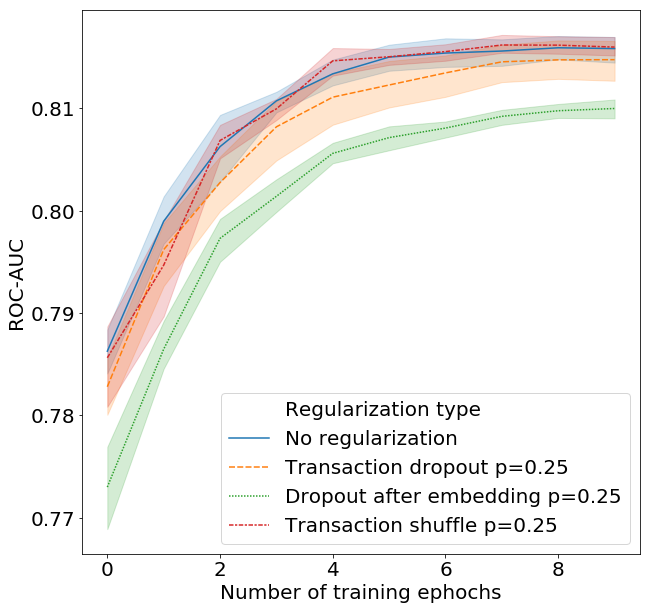
\includegraphics[width=0.46\textwidth]{figures/tmp-pic.png}
  \label{fig-emb-dim}
\end{figure}


\todo[inline]{provide plot of embedding dimensionality vs quality}

\subsection{Results} \label{sec-res}

\subsubsection{Comparison with baselines} \label{sec-res-baselines}

As shown in Table \ref{tab-age-pred} and Table \ref{tab-sex-pred} our method generates sequence embeddings of livestream data that achieve strong performance, comparable to performance on manually crafted features when used on downstream tasks. Also fine-tuned representations obtained by our method achieve state-of-the-art performance on both bank transactions datasets, outperforming all previous learning methods by a significant margin.

\todo[inline]{insert correct numbers}
\todo[inline]{insert CPC results}

\begin{table}[ht]
\caption{Age group prediction results}
\begin{tabular}{ | m{18em} |  m{6em} | }
\hline
\textbf{Method} & \textbf{Accuracy $\pm 95\%$} \\
\hline
\textbf{LightGBM on hand-crafted features} & $0.626 \pm 0.004$ \\
\textbf{LightGBM on Metric Learning embeddings} & $0.616 \pm 0.006$ \\
\textbf{LightGBM on both hand-crafted features and Metric Learning embeddings} & $0.632 \pm 0.007$ \\
\textbf{Supervised learning} & $0.628 \pm 0.010$  \\
\textbf{Fine-tuning} & \pmb{$0.643 \pm 0.007$}  \\
\hline
\end{tabular}
\label{tab-age-pred}
\end{table}

\begin{table}[ht]
\caption{Gender prediction results}
\begin{tabular}{ | m{18em} |  m{6em} | }
\hline
\textbf{Method} & \textbf{AUROC $\pm 95\%$} \\
\hline
\textbf{LightGBM on hand-crafted features} & $0.875 \pm 0.004$ \\
\textbf{LightGBM on Metric Learning embeddings} & $0.865 \pm 0.004$ \\
\textbf{LightGBM on both hand-crafted features and Metric Learning embeddings} & $0.878 \pm 0.004$ \\
\textbf{Supervised learning} & $0.871 \pm 0.007$  \\
\textbf{Fine-tuning} & \pmb{$0.883 \pm 0.003$} \\
\hline
\end{tabular}
\label{tab-sex-pred}
\end{table}

\subsubsection{Semi-supervised setup} \label{sec-semi}

In semi-supervised setting in addition to baselines (see Section \ref{sec-baselines}) we compared our method with pseudo-labeling (\cite{lee2013pseudo}). We used only part of available target labels for the semi-supervised experiment. As you can see in figure \ref{fig-semi}, the lesser the number of available labels the larger the gap in performance between our method and others.

\todo[inline]{Recreate image with larger fonts}

\begin{figure}[ht]
  \caption{Donwstream task quality for different dataset sizes}
  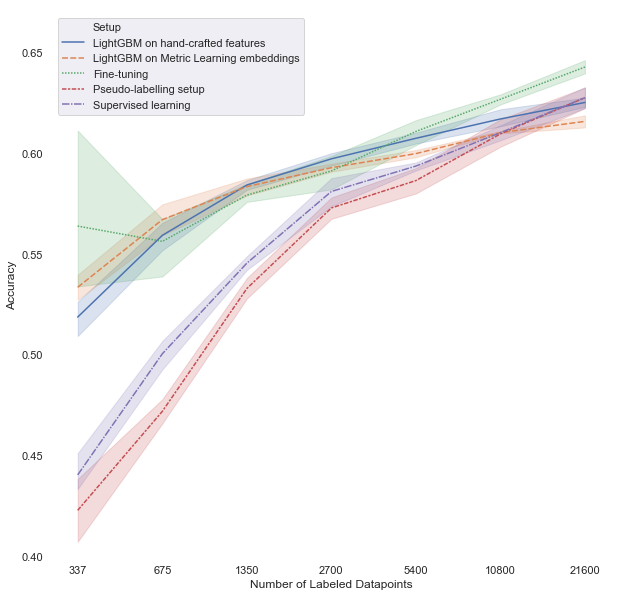
\includegraphics[width=0.46\textwidth]{figures/semi_supervised_setup.png}
  \label{fig-semi}
\end{figure}

\section{Conclusions} \label{sec-conclusions}

In this paper we proposes a novel method of self-supevised learning for live-stream data. Our method can be used to produce embeddings of complex event sequiences which can be effectively used in various downstream tasks. Also, our method can be used for pre-training in semi-supervised setting.

As we demonstrate in previous section our approach achieves strong performance on several downstream tasks. It outperforms both classical machine learning baselines on hand-crafted features and neural network based approaches.

In semi-supevised setting, where the number of labelled data is limited our method demonstrate even stronger results, it outperforms other methods by significant margin.

Our method of generating embeddings is convenient for production usage. For some encoder architectures (see Section \ref{sec-enc-arch} it is possible to update already calculated embeddings when additional data is arrived.

\bibliographystyle{ACM-Reference-Format}
\bibliography{sigconf}

\end{document}
